\documentclass[a5paper, 10pt]{tekst}

\usepackage{titlesec}
\usepackage{indentfirst}

\begin{document}
	\thispagestyle{empty}
	\onehalfspacing
	\titleformat*{\section}{\sffamily\bfseries}
	\sffamily
	
	\begin{center}
		\Huge \f{地震}{じしん}が\f{起}{お}こったら、その2
	\end{center}
	\vspace{2em}
	
	{\Large\sloppy
		\section{\p{\f{家}{いえ}に}\p{\f{帰}{かえ}る}\p{とき}}		\p{大きな}\p{\f{地震}{じしん}が}\p{\f{起}{お}こると、}\p{\f{電車}{でんしゃ}や}\p{バスなどが}\p{\f{止}{と}まる}\p{ことが}\p{あります。}\p{\f{急}{いそ}いで}\p{\f{家}{いえ}に}\p{\f{帰}{かえ}ろうと}\p{しないで、}\p{\f{会社}{かいしゃ}や}\p{\f{学校}{がっこう}など}\p{\f{安全}{あんぜん}な}\p{\f{場所}{ばしょ}で}\p{しばらく}\p{\f{待}{ま}って}\p{ください。}\p{\f{大勢}{おおぜい}の}\p{\f{人}{ひと}が}\p{\f{同}{おな}じ}\p{\f{時間}{じかん}に}\p{\f{帰}{かえ}ろうと}\p{すると、}\p{\f{道}{みち}や}\p{\f{駅}{えき}などが}\p{\f{混}{こ}んで}\p{\f{危険}{きけん}だからです。}\p{テレビや}\p{インターネットなどで}\p{\f{調}{しら}べて、}\p{\f{安全}{あんぜん}だと}\p{わかってから}\p{\f{帰}{かえ}りましょう。}
		
		\section{\p{\f{家族}{かぞく}や}\p{\f{友達}{ともだち}に}\p{\f{連絡}{れんらく}}\p{する}\p{とき}}
		\begin{figure}[h]
			\centering
			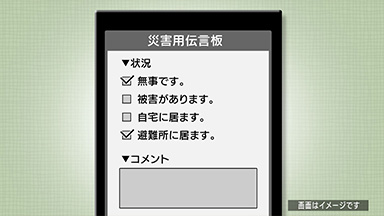
\includegraphics[width=0.5\linewidth]{figures/2017_earthquake5.jpg}		
		\end{figure}
		\p{\f{地震}{じしん}の}\p{あとは}\p{\f{大勢}{おおぜい}の}\p{\f{人}{ひと}が}\p{\f{電話}{でんわ}を}\p{\f{使}{つか}う}\p{ため、}\p{\f{家族}{かぞく}や}\p{\f{友達}{ともだち}に}\p{\f{連絡}{れんらく}}\p{しにくく}\p{なります。}\p{\f{電話}{でんわ}}\p{\f{番号}{ばんごう}}\p{171の}\p{「\f{災害}{さいがい}\f{用}{よう}}\p{\f{伝言}{でんごん}}\p{ダイヤル」を}\p{\f{使}{つか}うと、}\p{\f{会話}{かいわ}は}\p{できなくても}\p{メッセージを}\p{\f{録音}{ろくおん}}\p{したり、}\p{\f{聞}{き}いたり}\p{する}\p{ことが}\p{できます。}\p{\f{携帯}{けいたい}}\p{\f{電話}{でんわ}}\p{\f{会社}{がいしゃ}の}\p{「\f{災害}{さいがい}\f{用}{よう}}\p{\f{伝言}{でんごん}\f{板}{ばん}」などでも}\p{メッセージを}\p{\f{送}{おく}る}\p{ことが}\p{できますから、}\p{\f{使}{つか}い\f{方}{かた}を}\p{\f{調}{しら}べて}\p{おきましょう。}
		
		\section{\p{\f{家}{いえ}で}\p{\f{生活}{せいかつ}が}\p{できない}\p{とき}}
		\p{\f{建物}{たてもの}が}\p{\f{壊}{こわ}れたり}\p{して}\p{\f{家}{いえ}で}\p{\f{生活}{せいかつ}が}\p{できなく}\p{なった}\p{\f{場合}{ばあい}、}\p{\f{市}{し}や}\p{\f{町}{まち}などが}\p{\f{決}{き}めた}\p{「\f{避難}{ひなん}\f{所}{しょ}」に}\p{しばらく}\p{いる}\p{ことが}\p{できます。}\p{\f{大勢}{おおぜい}の}\p{\f{人}{ひと}と}\p{\f{一緒}{いっしょ}に}\p{\f{生活}{せいかつ}を}\p{しますから、}\p{\f{健康}{けんこう}に}\p{\f{気}{き}を}\p{つけましょう。}
		
		\p{\f{狭}{せま}い}\p{\f{場所}{ばしょ}で}\p{\f{長}{なが}い}\p{\f{時間}{じかん}}\p{\f{体}{からだ}を}\p{\f{動}{うご}かさないと、}\p{「エコノミー}\p{クラス}\p{\f{症候}{しょうこう}}\p{\f{群}{ぐん}」と}\p{いう}\p{\f{病気}{びょうき}に}\p{なる}\p{ことも}\p{あります。}\p{車の}\p{中で}\p{\f{生活}{せいかつ}を}\p{する}\p{\f{人}{ひと}は}\p{\f{特}{とく}に}\p{\f{気}{き}を}\p{つけましょう。}
		
	}
	
	\clearpage
	\titleformat*{\section}{\rmfamily\bfseries}
	\rmfamily
	
	\section*{Vokabular}
	\begin{multicols}{2}[\centering \textbf{Bitno}]\noindent
		\dictentry{急いで\footnotemark}{いそいで}{\item u žurbi, žurno}{izraz}
		\dictentry{安全}{あんぜん}{\item sigurno}{imenica, na-pridjev}
		\dictentry{大勢}{おおぜい}{\item puno ljudi}{imenica, no-pridjev}
		\dictentry{危険}{きけん}{\item opasnost}{imenica, na-pridjev}
		\dictentry{連絡}{れんらく}{\item kontaktiranje}{imenica, suru-glagol}
		\dictentry{用}{よう}{\item posao, namjera}{imenica}
		\dictentry{会話}{かいわ}{\item razgovor}{imenica, suru-glagol}
		\dictentry{送る}{おくる}{\item poslati (stvar), ispratiti}{glagol {\upshape (五)}}
		\dictentry{生活}{せいかつ}{\item život (svakodnevni)}{imenica, suru-glagol}
		\dictentry{壊れる}{こわれる}{\item razbiti se, slomiti se}{glagol {\upshape (一)}}
		\dictentry{場合}{ばあい}{\item situacija, slučaj}{imenica(priložna)}
		\dictentry{決める}{きめる}{\item odlučiti}{glagol {\upshape (一)}}
		\dictentry{一緒に}{いっしょに}{\item zajedno}{prilog}
		\dictentry{気を付ける}{きをつける}{\item paziti}{izraz}
		\dictentry{特に}{とくに}{\item posebno}{prilog}
	\end{multicols}
	\begin{multicols}{2}[\centering \textbf{Ostalo}]
		\dictentry{家}{いえ}{\item kuća}{imenica}
		\dictentry{帰る}{かえる}{\item vratiti se}{glagol {\upshape (五)}}
		\dictentry{大きい}{おおきい}{\item velik}{i-pridjev}
		\dictentry{地震}{じしん}{\item potres}{imenica}
		\dictentry{起こる}{おこる}{\item dogoditi se}{glagol {\upshape (五)}}
		\dictentry{電車}{でんしゃ}{\item vlak}{imenica}
		\dictentry{止まる}{とまる}{\item stati}{glagol {\upshape (五)}}
		\dictentry{会社}{かいしゃ}{\item tvrtka}{imenica}
		\dictentry{学校}{がっこう}{\item škola}{imenica}
		\dictentry{場所}{ばしょ}{\item mjesto}{imenica}
		\dictentry{待つ}{まつ}{\item čekati}{glagol {\upshape (五)}}
		\dictentry{同じ}{おなじ}{\item isto}{imenica, prilog}
		\dictentry{時間}{じかん}{\item vrijeme}{imenica}
		\dictentry{道}{みち}{\item put, cesta}{imenica}
		\dictentry{駅}{えき}{\item stanica}{imenica, brojač}
		\dictentry{込む}{こむ}{\item nakrcati se, biti krcat}{glagol {\upshape (五)}}
		\dictentry{調べる}{しらべる}{\item istražiti}{glagol {\upshape (一)}}
		\dictentry{家族}{かぞく}{\item obitelj}{imenica }
		\dictentry{友達}{ともだち}{\item prijatelj}{ imenica}
		\dictentry{電話}{でんわ}{\item telefon (-ski poziv)}{imenica, suru-glagol}
		\dictentry{使う}{つかう}{\item koristiti}{glagol {\upshape (五)}}
		\dictentry{電話番号}{でんわばんごう}{\item broj mobitela}{imenica}
		\dictentry{災害}{さいがい}{\item katastrofa}{imenica}
		\dictentry{伝言}{でんごん}{\item poruka}{imenica, suru-glagol}
		\dictentry{録音}{ろくおん}{\item audio sadržaj}{imenica, suru-glagol}
		\dictentry{聞く}{きく}{\item čuti}{glagol {\upshape (五)}}
		\dictentry{携帯電話会社}{けいたいでんわがいしゃ}{\item telefonska kompanija}{imenica}
		\dictentry{伝言板}{でんごんばん}{\item ploča za poruke}{imenica}
		\dictentry{使い方}{つかいかた}{\item način korištenja}{imenica}
		\dictentry{建物}{たてもの}{\item građevina}{imenica}
		\dictentry{市}{し}{\item grad}{imenica, sufiks}
		\dictentry{町}{まち}{\item manji grad}{imenica}
		\dictentry{避難所}{ひなんじょ}{\item sklonište}{imenica}
		\dictentry{健康}{けんこう}{\item zdravlje}{imenica, na-pridjev}
		\dictentry{狭い}{せまい}{\item skučeno, usko}{i-pridjev}
		\dictentry{長い}{ながい}{\item dugačko}{i-pridjev}
		\dictentry{体}{からだ}{\item tijelo}{imenica}
		\dictentry{動かす}{うごかす}{\item pomaknuti}{glagol {\upshape (五)}}
		\dictentry{エコノミークラス症候群}{えこのみいくらすしょうこうぐん}{\item sindrom ekonomske klase}{imenica}
		\dictentry{病気}{びょうき}{\item bolest}{imenica, no-pridjev, suru-glagol}
		\dictentry{車}{くるま}{\item automobil}{imenica}
		\dictentry{中}{なか}{\item unutar, sredina}{imenica}
	\end{multicols}
	\footnotetext{急いで je u osnovi て oblik od 急ぐ, ali se često u rječniku navodi kao izraz za sebe zato što se često koristi u ovom obliku}
	\clearpage
	
	\section*{Zadaci}
	\begin{enumerate} 
		\item Sažmite tekst u najviše dvije rečenice.\\[0.6em]
		\rule{\linewidth}{0.5pt}\\[0.6em]
		\rule{\linewidth}{0.5pt}\\[0.6em]
		\rule{\linewidth}{0.5pt}
		\item Razgovarajte o tekstu.
	\end{enumerate}
	
	\section*{Domaća zadaća}
	\begin{enumerate}
		\item Napišite kratku priču ili par rečenica koristeći riječi iz kutije ispod:
		\begin{center}
			\fbox{安全 ・ 連絡 ・ 会話 ・ 送る ・ 一緒に ・ 特に}
		\end{center}
		Rečenice ili tekst ne moraju nužno biti vezane uz samu vijest. 
		\item Odgovorite na pitanja:
		\begin{enumerate}[label=(\roman*)]
			\item \p{どう}\p{して}\p{\f{記事}{きじ}は}\p{\f{急}{いそ}いで}\p{\f{家}{いえ}に}\p{\f{帰}{かえ}る}\p{ことを}\p{お}\p{\f{勧}{すす}め}\p{しないのですか?}
			\item \p{どこで}\p{\f{情報}{じょうほう}を}\p{\f{集}{あつ}める}\p{ことが}\p{できますか?}
			\item \p{どの}\p{\f{様}{よう}に}\p{\f{家族}{かぞく}や}\p{\f{友達}{ともだち}と}\p{\f{連絡}{れんらく}を}\p{とる}\p{ことが}\p{できますか?}
			\item \p{どう}\p{して}\p{\f{避難}{ひなん}\f{所}{じょ}に}\p{いる}\p{時}\p{\f{健康}{けんこう}に}\p{\f{気}{き}を}\p{\f{付}{つ}けなければ}\p{なりませんか?}
			\item \p{エコノミー}\p{クラス}\p{\f{症候}{しょうこう}}\p{\f{群}{ぐん}は}\p{どう}\p{いう}\p{\f{病気}{びょうき}なんですか?}
		\end{enumerate}		
		\item Nadopunite sljedeće rečenice riječima iz kutije ispod:
		\begin{center}
			\fbox{用 ・ 一緒に ・ 安全 ・ 特に ・ 壊れて ・ 急いで ・ 電話}
		\end{center}
		\begin{enumerate}[label=(\roman*)]
			\item \ansline{}\p{うちまで}\p{\f{武}{たけし}\f{君}{くん}を}\p{\f{連}{つ}れて}\p{くれ。}
			\item \p{ファイアーウォールが}\p{インターネットの\ansline{}を}\p{\f{保障}{ほしょう}}\p{する。}
			\item \p{\f{花子}{はなご}ちゃんは}\p{\f{警察}{けいさつ}に\ansline{}}\p{します。}
			\item \p{\f{鈴木}{すずき}}\p{\f{先生}{せんせい}に}\p{\f{何}{なん}の\ansline{}?}
			\item \p{\f{酷}{ひど}い}\p{\f{目}{め}に}\p{あいたく}\p{ないなら、}\p{\f{武}{たけし}\f{君}{くん}と\ansline{}に}\p{\f{関}{かか}わらない}\p{\f{方}{ほう}が}\p{いいです。}
			\item \p{\f{貴重}{きちょう}な}\p{\f{花瓶}{かびん}が\ansline{}}\p{\f{武}{たけし}\f{君}{くん}は}\p{\f{困}{こま}って}\p{いる。}
			\item \p{\f{親}{おや}と\ansline{}}\p{\f{住}{す}むのが}\p{とても}\p{\f{不便}{ふべん}です。}
		\end{enumerate}
	\end{enumerate}
\end{document}